\chapter{Proton-NMR}\label{ch:g12:proton-nmr}

In een ziekenhuis ligt een patiënt in de ring van een MRI-scanner, en op
het scherm verschijnt een beeld van de zachte weefsels van het lichaam,
opgebouwd uit de antwoorden van de waterstofkernen in zijn water en
vetten. In een scheikundelaboratorium wordt een glazen buisje met een
paar milligram van een verbinding in de opening van een sterke magneet
neergelaten, en er verschijnt een spectrum dat op dezelfde manier tot
stand komt: een sterke magneet, een radiosignaal, en waterstofkernen die
daarop antwoorden. In de spectrometer van de scheikundige antwoordt elke
waterstofkern een beetje anders, afhankelijk van zijn buren, en het
spectrum is een kaart van de waterstofatomen van het \omterm{def:g7:atoms-and-molecules:molecule}{molecuul}.

\begin{recall}
Een \omterm{def:g11:infrared:spectrum}{infraroodspectrum} laat zien welke bindingen een \omterm{def:g7:atoms-and-molecules:molecule}{molecuul} bevat
(\cref{ch:g11:infrared}). \omterm{def:g11:functional-groups:functional-group}{Karakteristieke groepen}, families en \omterm{def:g11:organic-skeletons:isomer}{isomeren}
(\cref{ch:g11:functional-groups}, \cref{ch:g11:organic-skeletons}).
\end{recall}

\begin{omfigure}
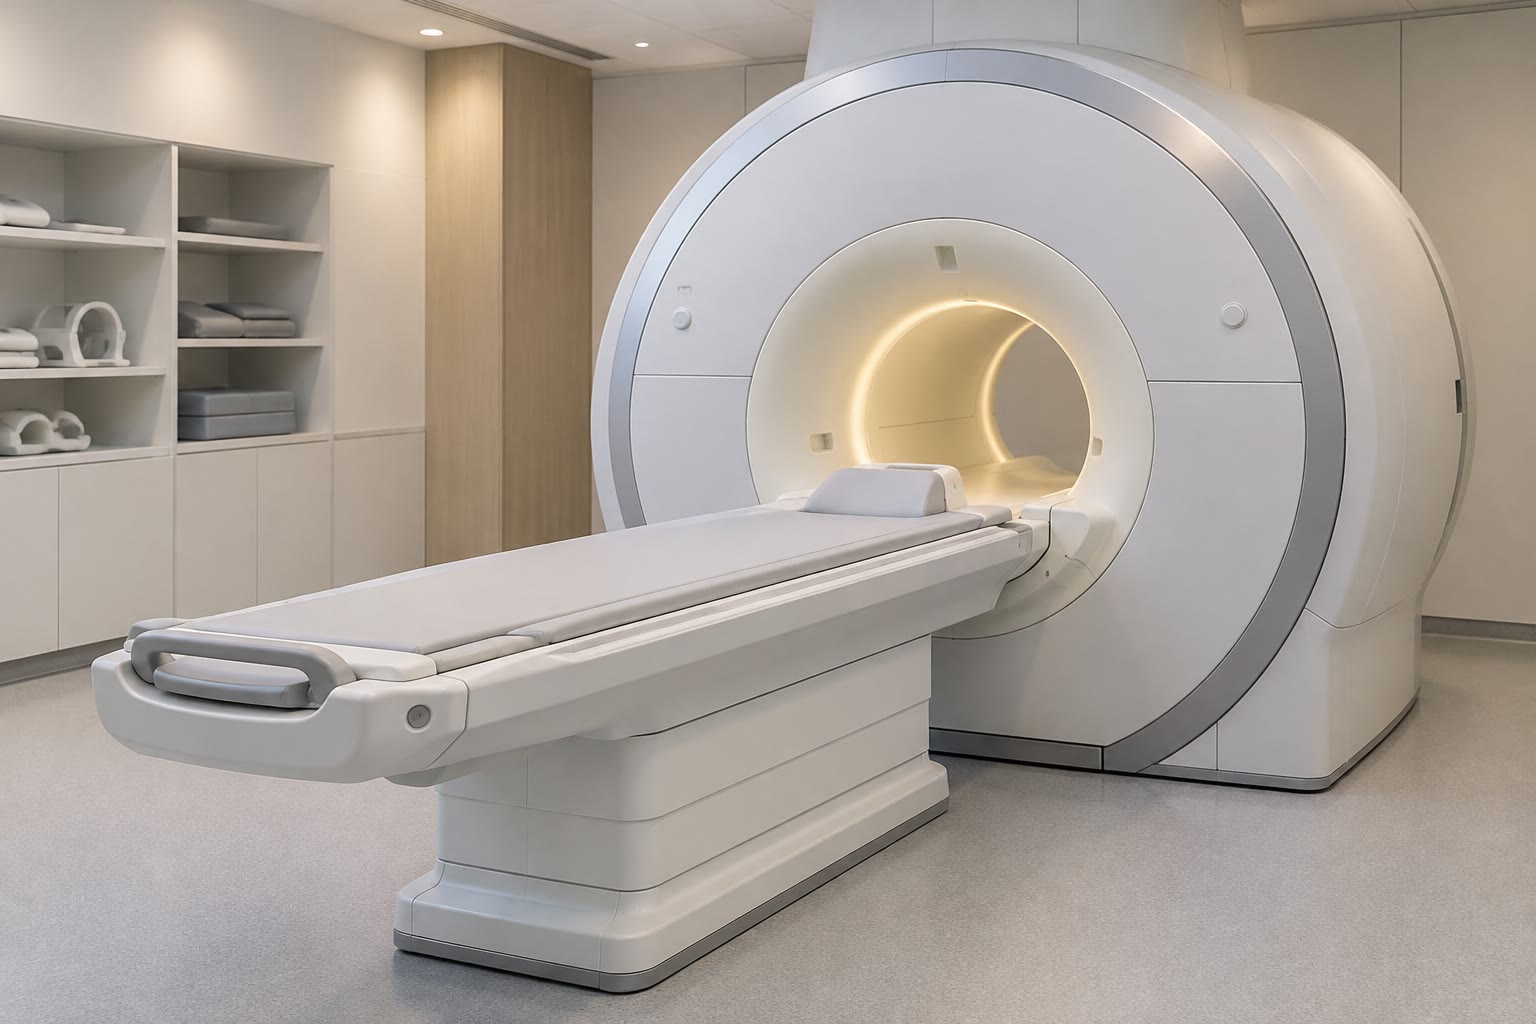
\includegraphics[width=0.48\linewidth]{images/book1/ai/g12-mri-room.jpg}

{\small Een MRI-scanner: dezelfde natuurkunde als in de NMR-spectrometer
van de scheikundige.}
\end{omfigure}

\section{Protonen in een magnetisch veld}

De kern van een waterstofatoom is één enkel \omterm{def:g9:inside-the-atom:proton}{proton}. In een sterk
magnetisch veld absorbeert het radiogolven van een precieze frequentie;
hoe en waarom dat gebeurt, hoort bij de natuurkunde en is hier niet
nodig. Voor de scheikundige telt dat de \omterm{def:g9:inside-the-atom:nucleus}{elektronen} rond een \omterm{def:g9:inside-the-atom:proton}{proton} het
een beetje afschermen van het veld, en dat die afscherming afhangt van de
\omterm{def:g7:atoms-and-molecules:atom}{atomen} in de buurt: een \omterm{def:g9:inside-the-atom:proton}{proton} naast een elektronegatief zuurstofatoom,
dat \omterm{def:g9:inside-the-atom:nucleus}{elektronen} naar zich toe trekt, absorbeert bij een iets andere
frequentie dan een \omterm{def:g9:inside-the-atom:proton}{proton} in een koolwaterstofketen. De verschillen zijn
heel klein, een paar miljoenste van de frequentie, en worden opgegeven in
delen per miljoen.

\begin{omfigure}
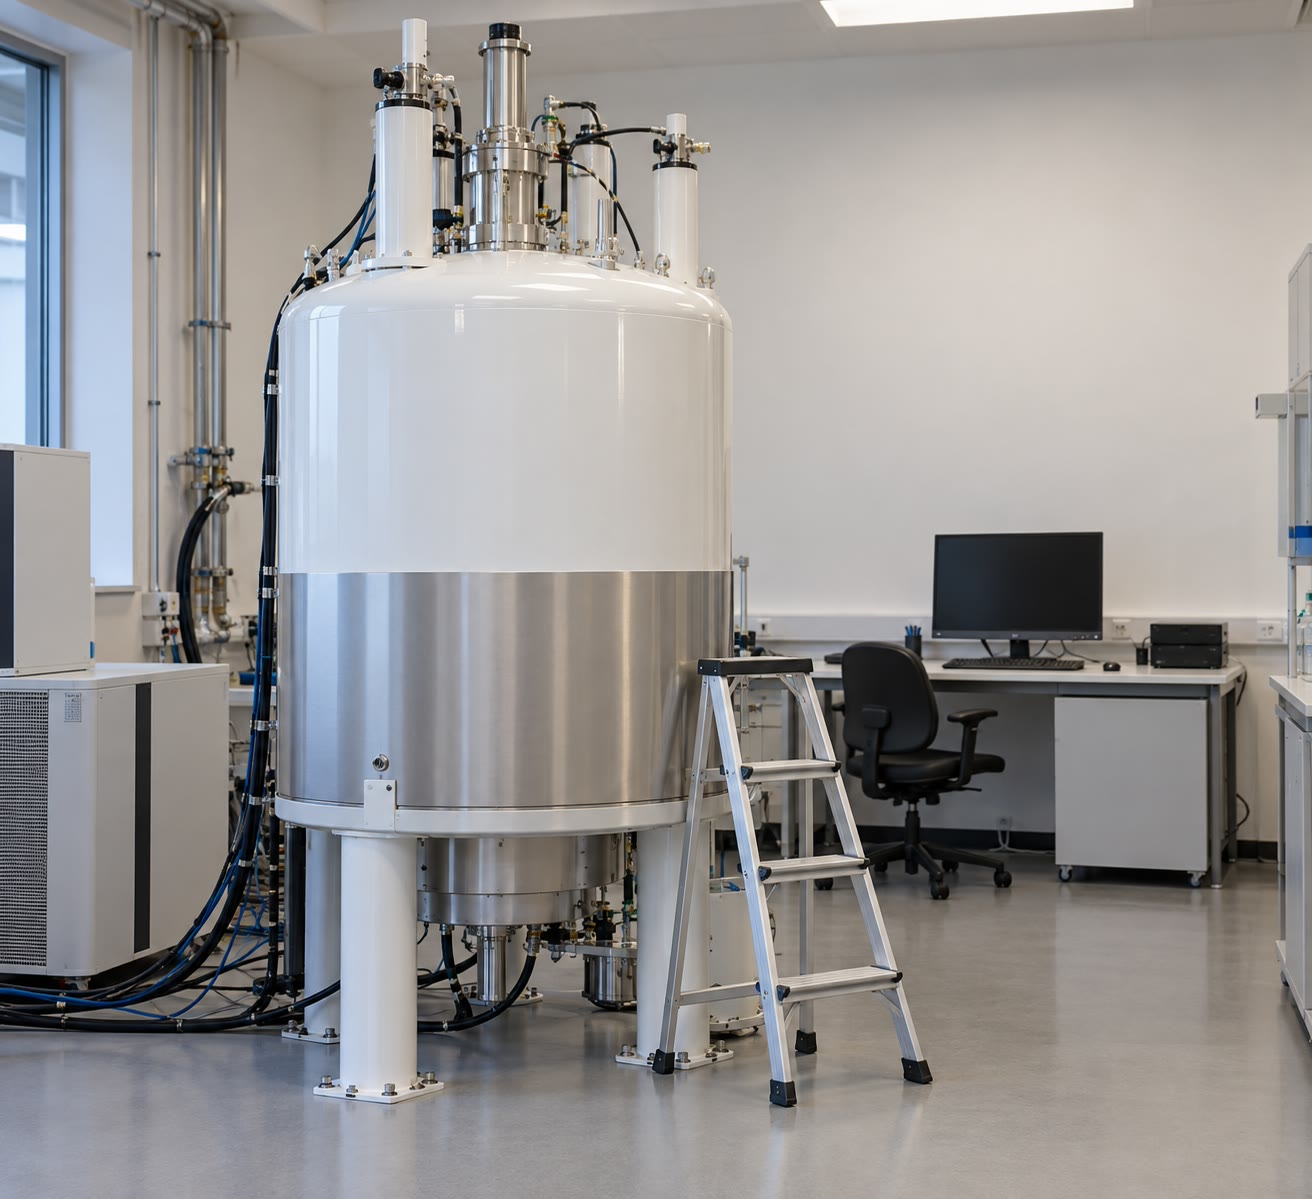
\includegraphics[width=0.42\linewidth]{images/book1/ai/g12-nmr-magnet.jpg}

{\small De magneet van een NMR-spectrometer.}
\end{omfigure}

\begin{definition}[NMR-spectrum, chemische verschuiving]\label{def:g12:proton-nmr:spectrum}
Een proton-\emph{NMR-spectrum}\index{NMR-spectrum} (nucleaire magnetische
resonantie, of kernspinresonantie) laat de signalen zien die de
waterstofkernen van een verbinding absorberen. De plaats van een signaal
is zijn \emph{chemische verschuiving}\index{chemische verschuiving}
$\delta$, in delen per miljoen (\si{ppm}),
gemeten vanaf het signaal van een referentieverbinding, tetramethylsilaan
\ce{Si(CH3)4} (TMS), dat op $\delta = 0$ gezet wordt. De $\delta$-as wordt
van rechts naar links oplopend getekend.
\end{definition}

\begin{proposition}[De verschuiving hangt af van de buren]\label{prop:g12:proton-nmr:shift}
% ledger: nmrr:CH3, nmrr:CH2, nmrr:allylic, nmrr:ketone, nmrr:halide, nmrr:alcohol, nmrr:vinylic, nmrr:aryl, nmrr:aldehyde, nmrr:acid
De \omterm{def:g12:proton-nmr:spectrum}{chemische verschuiving} van een \omterm{def:g9:inside-the-atom:proton}{proton} hangt af van de \omterm{def:g7:atoms-and-molecules:atom}{atomen} in zijn
buurt: hoe dichter het bij een elektronegatief \omterm{def:g7:atoms-and-molecules:atom}{atoom} of een \omterm{def:g10:lewis-and-shape:multiple-bond}{dubbele
binding} zit, hoe groter zijn verschuiving. Typische gebieden, in
\si{ppm}:
\begin{center}
\small
\begin{tabular}{ll@{\qquad}ll}
\hline
omgeving & $\delta$ & omgeving & $\delta$ \\
\hline
\ce{CH3} in een keten & 0.7--1.3 & \ce{H-C-O} (\omterm{def:g11:functional-groups:alcohol}{alcohol}, ether, \omterm{def:g11:functional-groups:carboxylic-acid}{ester}) & 3.3--4.5 \\
\ce{CH2} in een keten & 1.2--1.6 & \ce{H-C=C} & 4.5--6.5 \\
\ce{H-C-C=C} & 1.6--2.2 & H aan een benzeenring & 6.5--8.0 \\
\ce{H-C-C=O} & 2.0--2.4 & \omterm{def:g11:functional-groups:carbonyl}{aldehyde} \ce{-CHO} & 9.7--10.0 \\
\ce{H-C-X} (\omterm{def:g10:electron-shells:family}{halogeen}) & 2.5--4.0 & zuur \ce{-COOH} & 11.0--12.0 \\
\hline
\end{tabular}
\end{center}
\end{proposition}

\begin{proof}
Gemeten aan veel verbindingen (ledger). Een elektronegatieve buur trekt
\omterm{def:g9:inside-the-atom:nucleus}{elektronen} weg van het \omterm{def:g9:inside-the-atom:proton}{proton}, dat minder afgeschermd is en bij een
grotere verschuiving absorbeert.
\end{proof}

\begin{omfigure}
\begin{tikzpicture}[font=\small, x=0.75cm, y=0.5cm]
  % delta axis reversed: x = 12 - delta
  \draw[->] (0,0) -- (12.4,0) node[right] {};
  \foreach \d in {12,11,10,9,8,7,6,5,4,3,2,1,0}
    \draw ({12-\d},0) -- ({12-\d},-0.2) node[below, font=\footnotesize] {\d};
  \node[below=14pt] at (6,-0.3) {$\delta$ (\si{ppm})};
  \foreach \a/\b/\y/\c/\l in {
      11.0/12.0/1/omThm/{\ce{COOH}},
      9.7/10.0/2/omThm/{\ce{CHO}},
      6.5/8.0/1/black!60/{benzeenring},
      4.5/6.5/2/omMeth/{\ce{C=C-H}},
      3.3/4.5/3/omDef/{\ce{H-C-O}},
      2.0/2.4/4/omProp/{\ce{H-C-C=O}},
      0.7/1.6/5/black!45/{\ce{CH3}, \ce{CH2} van ketens}} {
    \fill[\c, rounded corners=1pt] ({12-\b},{\y-0.3}) rectangle ({12-\a},{\y+0.3});
    \node[anchor=west, font=\footnotesize] at ({12-\a+0.1},\y) {\l};
  }
  \draw[thick] (12,0) -- (12,0.6) node[above, font=\footnotesize] {TMS};
\end{tikzpicture}

{\small Waar \omterm{def:g9:inside-the-atom:proton}{protonen} absorberen, per omgeving. \omterm{def:g9:inside-the-atom:proton}{Protonen} dicht bij
zuurstof, bij een \omterm{def:g10:lewis-and-shape:multiple-bond}{dubbele binding} of bij een zuurgroep verschijnen links
in het spectrum.}
\end{omfigure}

\begin{inthelab}[Een NMR-buisje klaarmaken]
Een paar milligram van de verbinding wordt opgelost in ongeveer
\qty{0.6}{mL} van een \omterm{def:g6:solutions-and-solubility:solute}{oplosmiddel} waarvan de waterstofatomen vervangen
zijn door deuterium (\ce{CDCl3}, gedeutereerd chloroform), dat geen
signaal geeft; als referentie komt er een spoortje TMS bij. De oplossing
wordt in een dun glazen buisje gefiltreerd, dat wordt afgesloten, van een
etiket voorzien en in de magneet neergelaten.
\end{inthelab}

\section{Equivalente protonen}

\begin{definition}[Equivalente protonen]\label{def:g12:proton-nmr:equivalent}
\omterm{def:g9:inside-the-atom:proton}{Protonen} zijn \emph{equivalente protonen}\index{equivalente protonen} als
ze in het \omterm{def:g7:atoms-and-molecules:molecule}{molecuul} dezelfde omgeving hebben, zodat ze bij dezelfde
verschuiving absorberen. Elke groep equivalente \omterm{def:g9:inside-the-atom:proton}{protonen} geeft één
signaal. De drie \omterm{def:g9:inside-the-atom:proton}{protonen} van een \ce{CH3}-groep zijn altijd equivalent.
\end{definition}

\begin{example}[Groepen tellen]\label{ex:g12:proton-nmr:groups}
Propanon, \ce{CH3-CO-CH3}, heeft zes \omterm{def:g9:inside-the-atom:proton}{protonen} maar één groep: de twee
\ce{CH3} zijn gelijk, één aan elke kant van de \ce{C=O}. Ethanol,
\ce{CH3-CH2-OH}, heeft drie groepen (\ce{CH3}, \ce{CH2}, \ce{OH}), en
ethylethanoaat, \ce{CH3-CO-O-CH2-CH3}, ook drie: de \ce{CH3} naast de
\ce{C=O}, de \ce{CH2} naast de \ce{O}, en de \ce{CH3} aan het
eind.
\end{example}

\section{Integratie}

\begin{definition}[Integratiecurve]\label{def:g12:proton-nmr:integration}
De \emph{integratiecurve}\index{integratiecurve} van een \omterm{def:g12:proton-nmr:spectrum}{NMR-spectrum} is
een curve, boven de signalen getekend, die bij elk signaal een trede
omhoog gaat: de hoogte van elke trede is evenredig met het aantal
\omterm{def:g9:inside-the-atom:proton}{protonen} dat dat signaal geeft.
\end{definition}

\begin{example}[De treden aflezen]\label{ex:g12:proton-nmr:steps}
In het spectrum van ethanol meten de treden boven de drie signalen 2,
1 en 3 eenheden, van links naar rechts: \ce{CH2}, \ce{OH} en \ce{CH3}.
Alleen de verhoudingen tellen: treden van 12, 6 en 18 mm zeggen hetzelfde.
\end{example}

\section{Multipliciteit en de \texorpdfstring{$n+1$}{n+1}-regel}


\begin{definition}[Multiplet, $n+1$-regel]\label{def:g12:proton-nmr:multiplet}
Een signaal is vaak gesplitst in een aantal dicht bij elkaar liggende
lijnen: een \emph{multiplet}\index{multiplet}
(singlet, doublet, triplet, kwartet, \dots{} voor 1, 2, 3, 4 lijnen). Volgens de
\emph{$n+1$-regel}\index{n+1-regel@$n+1$-regel} geeft een groep
\omterm{def:g12:proton-nmr:equivalent}{equivalente protonen} waarvan de naburige koolstofatomen samen $n$
\omterm{def:g9:inside-the-atom:proton}{protonen} dragen die er niet equivalent mee zijn, een signaal van $n+1$
lijnen, met intensiteiten in de verhoudingen van de driehoek van
Pascal.
\end{definition}

\begin{proposition}[Splitsing door buren]\label{prop:g12:proton-nmr:n-plus-one}
In een \omterm{def:g7:atoms-and-molecules:molecule}{molecuul} \ce{CH3-CH2-X} (X zonder waterstof) is het signaal van
\ce{CH3} een triplet (2 naburige \omterm{def:g9:inside-the-atom:proton}{protonen}) en dat van \ce{CH2} een
kwartet (3 naburige \omterm{def:g9:inside-the-atom:proton}{protonen}). \omterm{def:g9:inside-the-atom:proton}{Protonen} die aan een zuurstof- of
stikstofatoom gebonden zijn, geven meestal een singlet en splitsen hun
buren niet.
\end{proposition}

\begin{proof}
Aangenomen: elk naburig \omterm{def:g9:inside-the-atom:proton}{proton} verschuift het signaal een klein beetje
omhoog of omlaag, afhankelijk van zijn eigen toestand, en de combinaties
geven $n+1$ lijnen; de natuurkunde daarachter wordt uitgelegd in het
deel voor het eerste universiteitsjaar. \omterm{def:g9:inside-the-atom:proton}{Protonen} aan O of N worden snel
tussen \omterm{def:g7:atoms-and-molecules:molecule}{moleculen} uitgewisseld, waardoor hun effect wegmiddelt.
\end{proof}

\begin{omfigure}
\begin{tikzpicture}[font=\small]
  % de driehoek van Pascal
  \foreach \r/\vals in {0/{1}, 1/{1,1}, 2/{1,2,1}, 3/{1,3,3,1}, 4/{1,4,6,4,1}} {
    \foreach \v [count=\i from 0] in \vals
      \node at ({\i*0.7 - \r*0.35}, {-\r*0.55}) {\v};
    \node[anchor=east, font=\footnotesize, black!60] at (-2.0,{-\r*0.55}) {$n = \r$};
  }
  % multipletten
  \begin{scope}[xshift=4.2cm, yshift=-2.4cm]
    \foreach \x/\name/\hs in {0/singlet/{1}, 1.4/doublet/{1,1}, 3.0/triplet/{1,2,1},
                              4.9/kwartet/{1,3,3,1}} {
      \foreach \h [count=\i from 0] in \hs {
        \draw[very thick, omDef] ({\x + \i*0.22},0) -- ({\x + \i*0.22},{\h*0.55});
      }
      \node[anchor=north, font=\footnotesize] at ({\x+0.3},-0.1) {\name};
    }
  \end{scope}
\end{tikzpicture}

{\small De driehoek van Pascal geeft de relatieve intensiteiten van de
$n+1$ lijnen van een signaal dat door $n$ naburige \omterm{def:g9:inside-the-atom:proton}{protonen} gesplitst
wordt: 1:1, 1:2:1, 1:3:3:1.}
\end{omfigure}

\begin{omfigure}
\newcommand{\nmrpanel}[4]{% bestandsdeel, titel, xmax, ymax
\begin{tikzpicture}
\begin{axis}[width=\linewidth, height=4.2cm, x dir=reverse, xmin=0,
    xmax=#3, ymin=0, ymax=#4, ytick=\empty, axis y line=none,
    axis x line*=bottom, xlabel={$\delta$ (\si{ppm})},
    tick label style={font=\scriptsize}, label style={font=\scriptsize},
    title={\small #2}, title style={yshift=-3pt}]
  \addplot[omDef, thin] table[x=delta, y=I] {figdata/out/grade-12-proton-nmr-#1.dat};
  \addplot[omProp, thick] table[x=delta, y expr=0.15+\thisrow{integral}*0.11]
    {figdata/out/grade-12-proton-nmr-#1.dat};
\end{axis}
\end{tikzpicture}}
\begin{minipage}{0.49\linewidth}\nmrpanel{a}{A: ethanol}{5}{1.15}\end{minipage}\hfill
\begin{minipage}{0.49\linewidth}\nmrpanel{b}{B: ethylethanoaat}{5}{1.15}\end{minipage}

\begin{minipage}{0.49\linewidth}\nmrpanel{c}{C: propanon}{5}{1.15}\end{minipage}\hfill
\begin{minipage}{0.49\linewidth}\nmrpanel{e}{D: methylethanoaat}{5}{1.15}\end{minipage}

\begin{minipage}{\linewidth}\nmrpanel{d}{E: propaanzuur}{12.5}{1.15}\end{minipage}

{\small \omterm{def:g12:proton-nmr:spectrum}{Proton-NMR-spectra} (blauw) met hun \omterm{def:g12:proton-nmr:integration}{integratiecurven} (oranje;
elke trede is evenredig met het aantal \omterm{def:g9:inside-the-atom:proton}{protonen} van het signaal eronder).
De verschuivingen zijn die van gemeten spectra in \ce{CDCl3}; de vorm en
de afstanden van de lijnen zijn getekend met een eenvoudig model.}
\end{omfigure}

\begin{example}[De spectra lezen]\label{ex:g12:proton-nmr:reading}
% ledger: nmr:ethylethanoate-OCH2, nmr:ethylethanoate-COCH3, nmr:ethylethanoate-CH3, nmr:ethanol-CH2, nmr:ethanol-CH3, nmr:ethanol-OH, nmr:acetone, nmr:propanoic-CH2, nmr:propanoic-CH3, nmr:propanoic-OH, nmr:meoac-OCH3, nmr:meoac-COCH3
Ethylethanoaat (B) geeft een kwartet van 2 \omterm{def:g9:inside-the-atom:proton}{protonen} bij \qty{4.12}{ppm}
(\ce{O-CH2}, naast zuurstof en naast een \ce{CH3}), een singlet van 3
\omterm{def:g9:inside-the-atom:proton}{protonen} bij \qty{2.04}{ppm} (\ce{CH3-C=O}, geen naburig \omterm{def:g9:inside-the-atom:proton}{proton}) en een
triplet van 3 \omterm{def:g9:inside-the-atom:proton}{protonen} bij \qty{1.26}{ppm} (\ce{CH3}, naast een
\ce{CH2}). Propanon (C) geeft één singlet van 6 \omterm{def:g9:inside-the-atom:proton}{protonen} bij
\qty{2.16}{ppm}. Propaanzuur (E) heeft een kwartet bij \qty{2.39}{ppm},
een triplet bij \qty{1.16}{ppm}, en een singlet ver naar links, bij
\qty{11.7}{ppm}: zijn zure \omterm{def:g9:inside-the-atom:proton}{proton}.
\end{example}

\section{Infrarood en NMR samen gebruiken}


\begin{method}[Een molecuul identificeren uit zijn IR- en NMR-spectrum]\label{met:g12:proton-nmr:identify}
\begin{enumerate}
  \item Stel uit de \omterm{def:g11:organic-skeletons:formulas}{molecuulformule} de lijst op van de mogelijke
        \omterm{def:g11:organic-skeletons:isomer}{isomeren} en hun \omterm{def:g11:functional-groups:functional-group}{karakteristieke groepen}.
  \item Infrarood: zoek een \ce{C=O}-band bij ongeveer
        \qty{1700}{cm^{-1}} en \ce{O-H}- of \ce{N-H}-banden; streep de
        \omterm{def:g11:organic-skeletons:isomer}{isomeren} door die niet passen.
  \item NMR: tel de signalen (groepen \omterm{def:g12:proton-nmr:equivalent}{equivalente protonen}), lees de
        integratie (\omterm{def:g9:inside-the-atom:proton}{protonen} per groep), de multipliciteiten (buren) en
        de verschuivingen (omgevingen) af.
  \item Zet de stukjes samen tot één structuur, en controleer die aan
        elke waarneming.
\end{enumerate}
\end{method}

\begin{example}[Twee isomeren \ce{C3H6O2}]\label{ex:g12:proton-nmr:isomers}
Propaanzuur \ce{CH3-CH2-COOH} en methylethanoaat \ce{CH3-CO-O-CH3}
zijn \omterm{def:g11:organic-skeletons:isomer}{isomeren}. In het infrarood laat alleen het zuur de zeer brede
\ce{O-H}-band zien. In de NMR (spectra E en D) geeft het zuur een
triplet, een kwartet en een singlet bij ongeveer \qty{11.7}{ppm}; de \omterm{def:g11:functional-groups:carboxylic-acid}{ester}
geeft twee singlets van elk 3 \omterm{def:g9:inside-the-atom:proton}{protonen},
bij 3.66 (\ce{O-CH3}) en \qty{2.05}{ppm} (\ce{CH3-C=O}), omdat geen enkel
koolstofatoom van de \omterm{def:g11:functional-groups:carboxylic-acid}{ester} \omterm{def:g9:inside-the-atom:proton}{protonen} draagt naast een ander koolstofatoom
met \omterm{def:g9:inside-the-atom:proton}{protonen}.
\end{example}

\section{Oefeningen}

\begin{exercise}[$\star$]\label{exo:g12:proton-nmr:1}
Hoeveel groepen \omterm{def:g12:proton-nmr:equivalent}{equivalente protonen}, en dus hoeveel signalen, geven deze
\omterm{def:g7:atoms-and-molecules:molecule}{moleculen}: methaan; ethaan \ce{CH3-CH3}; propaan; methanol
\ce{CH3-OH}; methoxymethaan \ce{CH3-O-CH3}?
\end{exercise}

\begin{exercise}[$\star$]\label{exo:g12:proton-nmr:2}
Een groep \omterm{def:g9:inside-the-atom:proton}{protonen} heeft 2 naburige \omterm{def:g9:inside-the-atom:proton}{protonen} aan het volgende
koolstofatoom. Hoeveel lijnen heeft zijn signaal, en in welke
verhoudingen? Dezelfde vraag voor 3 en voor 0 buren.
\end{exercise}

\begin{exercise}[$\star$]\label{exo:g12:proton-nmr:3}
Een spectrum heeft drie signalen met integratietreden van 15, 10 en
15 mm. Het \omterm{def:g7:atoms-and-molecules:molecule}{molecuul} heeft 8 \omterm{def:g9:inside-the-atom:proton}{protonen}. Hoeveel \omterm{def:g9:inside-the-atom:proton}{protonen} stelt elk signaal
voor?
\end{exercise}

\begin{exercise}[$\star$]\label{exo:g12:proton-nmr:4}
Waar verwacht je met de tabel van verschuivingen het signaal van een
\omterm{def:g9:inside-the-atom:proton}{proton} van een aldehydegroep? En van een \ce{CH3}-groep in een keten?
\end{exercise}

\begin{exercise}[$\star$]\label{exo:g12:proton-nmr:5}
Waarom kiest men als referentie TMS, waarvan alle \omterm{def:g9:inside-the-atom:proton}{protonen} equivalent
zijn? Waarom is het \omterm{def:g6:solutions-and-solubility:solute}{oplosmiddel} gedeutereerd?
\end{exercise}

\begin{exercise}[$\star\star$]\label{exo:g12:proton-nmr:6}
Voorspel het spectrum van chloorethaan \ce{CH3-CH2-Cl}: aantal signalen,
integratie, multipliciteiten, verschuivingen bij benadering.
\end{exercise}

\begin{exercise}[$\star\star$]\label{exo:g12:proton-nmr:7}
Voorspel het spectrum van propaan-2-ol, \ce{(CH3)2CH-OH}: in het
bijzonder de multipliciteit van het \ce{CH3}-signaal en van het
\ce{CH}-signaal (neem aan dat de \ce{OH} een singlet geeft en niet
splitst).
\end{exercise}

\begin{exercise}[$\star\star$]\label{exo:g12:proton-nmr:8}
Drie spectra: (a) één singlet; (b) een kwartet, een singlet en een
triplet, integraties 2:3:3; (c) een kwartet, een triplet en een singlet
ver naar links, integraties 2:3:1. Koppel ze aan ethylethanoaat, propanon
en propaanzuur.
\end{exercise}

\begin{exercise}[$\star\star$]\label{exo:g12:proton-nmr:9}
Leg met het diagram van de verschuivingen uit waarom de \ce{CH2} van
ethylethanoaat (\qty{4.12}{ppm}) ver links ligt van de \ce{CH3} van
dezelfde ethylgroep (\qty{1.26}{ppm}).
\end{exercise}

\begin{exercise}[$\star\star$]\label{exo:g12:proton-nmr:10}
Een verbinding \ce{C3H6O} heeft een sterke infraroodband bij
\qty{1715}{cm^{-1}} en één enkel NMR-singlet. Identificeer haar. Waarom
valt propanal af?
\end{exercise}

\begin{exercise}[$\star\star$]\label{exo:g12:proton-nmr:11}
Waarom is in het spectrum van ethanol het \ce{OH}-signaal een singlet, en
waarom verschijnt de \ce{CH2} als kwartet en niet als een ingewikkelder
signaal?
\end{exercise}

\begin{exercise}[$\star\star\star$]\label{exo:g12:proton-nmr:12}
Geef de structuren van vier \omterm{def:g11:organic-skeletons:isomer}{isomeren} \ce{C4H8O2} die \omterm{def:g11:functional-groups:carboxylic-acid}{esters} of zuren zijn
(butaanzuur, ethylethanoaat, methylpropanoaat, propylmethanoaat,
\dots) en voorspel voor elk het aantal NMR-signalen en hun
multipliciteiten.
\end{exercise}

\begin{exercise}[$\star\star\star$]\label{exo:g12:proton-nmr:13}
Een druppel zwaar water \ce{D2O} wordt geschud met een oplossing van
ethanol, en het spectrum wordt opnieuw opgenomen: één signaal verdwijnt.
Welk, en waarom? Hoe helpt dit om \ce{O-H}-protonen te herkennen?
\end{exercise}

\begin{exercise}[$\star\star\star$]\label{exo:g12:proton-nmr:14}
Een monster ethylethanoaat bevat wat ethanol. Welke extra signalen
verschijnen er in het spectrum? Als de integratie van het singlet bij
\qty{2.04}{ppm} 30 mm is en die van een klein extra triplet bij
\qty{1.23}{ppm} 3 mm, schat dan de verhouding tussen de hoeveelheden
ethanol en \omterm{def:g11:functional-groups:carboxylic-acid}{ester}.
\end{exercise}

\begin{exercise}[$\star\star\star$]\label{exo:g12:proton-nmr:15}
2-Methylpropaan-1-ol is \ce{(CH3)2CH-CH2-OH}. Voorspel zijn spectrum: de
signalen, hun integraties, en de multipliciteit van de \ce{CH3}- en
\ce{CH2}-signalen. Welk signaal heeft de meeste lijnen?
\end{exercise}

\section{Probleem: Het onbekende oplosmiddel}

\begin{problem}[{Weekendprobleem --- een fles \omterm{def:g6:solutions-and-solubility:solute}{oplosmiddel} met alleen
\ce{C4H8O2} op het etiket: wat zit erin, en hoe hoog is elke trede van
de \omterm{def:g12:proton-nmr:integration}{integratiecurve}?}]
\label{pb:g12:proton-nmr:1}
% ledger: nmr:ethylethanoate-OCH2, nmr:ethylethanoate-COCH3, nmr:ethylethanoate-CH3, ir:CO-ester, ir:OH-acid
Op een fles \omterm{def:g6:solutions-and-solubility:solute}{oplosmiddel} in een voorraadkast staat alleen
``\ce{C4H8O2}''. Het \omterm{def:g11:infrared:spectrum}{infraroodspectrum} laat een sterke band zien bij
\qty{1740}{cm^{-1}} en geen enkele band boven \qty{3100}{cm^{-1}}. Het
\omterm{def:g12:proton-nmr:spectrum}{NMR-spectrum} laat drie signalen zien: een kwartet bij \qty{4.12}{ppm},
een singlet bij \qty{2.04}{ppm} en een triplet bij \qty{1.26}{ppm}. De
\omterm{def:g12:proton-nmr:integration}{integratiecurve} stijgt in totaal \qty{72}{mm}.

\medskip
\noindent\textbf{Deel I --- De kandidaten.}
\begin{enumerate}
  \item Controleer dat \ce{C4H8O2} past bij een \omterm{def:g11:functional-groups:carboxylic-acid}{ester} of een \omterm{def:g11:functional-groups:carboxylic-acid}{carbonzuur}
        met alleen enkelvoudige bindingen in de keten.
  \item Geef de \omterm{def:g11:organic-skeletons:formulas}{beknopte structuurformules} en de namen van butaanzuur en
        van de drie \omterm{def:g11:functional-groups:carboxylic-acid}{esters} ethylethanoaat, methylpropanoaat en
        propylmethanoaat.
  \item Welke \omterm{def:g11:functional-groups:functional-group}{karakteristieke groep} hebben ze per paar gemeen?
\end{enumerate}

\medskip
\noindent\textbf{Deel II --- Infrarood.}
\begin{enumerate}[resume]
  \item Wat verraadt de band bij \qty{1740}{cm^{-1}}?
  \item Wat zou butaanzuur laten zien dat hier ontbreekt? Streep het
        door.
  \item Kan infrarood alleen kiezen tussen de drie \omterm{def:g11:functional-groups:carboxylic-acid}{esters}?
\end{enumerate}

\medskip
\noindent\textbf{Deel III --- NMR.}
\begin{enumerate}[resume]
  \item Hoeveel groepen \omterm{def:g12:proton-nmr:equivalent}{equivalente protonen} heeft de onbekende stof?
  \item Wat doen het kwartet en het triplet samen vermoeden?
  \item Wat zegt het singlet over de buren van zijn \omterm{def:g9:inside-the-atom:proton}{protonen}?
  \item Waarom ligt het kwartet bij een grote verschuiving?
  \item Voorspel het spectrum van methylpropanoaat
        \ce{CH3-CH2-CO-O-CH3} (signalen, multipliciteiten, verschuivingen
        bij benadering). Is dat de onbekende stof?
  \item Voorspel het spectrum van propylmethanoaat. Is dat de onbekende
        stof?
\end{enumerate}

\medskip
\noindent\textbf{Deel IV --- Identificatie en integratie.}
\begin{enumerate}[resume]
  \item Identificeer de onbekende stof en teken haar structuur, met bij
        elk signaal een label.
  \item Hoeveel \omterm{def:g9:inside-the-atom:proton}{protonen} stelt elk signaal voor?
  \item De totale integratie is \qty{72}{mm} voor 8 \omterm{def:g9:inside-the-atom:proton}{protonen}. Hoeveel
        millimeter is dat per \omterm{def:g9:inside-the-atom:proton}{proton}?
  \item Bereken de hoogte van de trede van het singlet en van het
        triplet.
  \item Controleer dat de drie treden samen \qty{72}{mm} zijn.
  \item Ethylethanoaat ruikt naar peerdrops: past dat bij de gevonden
        familie?
  \item Geef het eindantwoord: hoe hoog is de integratietrede van het
        kwartet?
\end{enumerate}
\end{problem}
